\chapter{A General Model for Large-Scale Networks} \label{system:chap}

In this chapter, we develop the system model that will be used for the rest of this dissertation. We first present a general framework describing large-scale networks in the context of our investigation, and then address particular details and the state of the art for both access control and user scheduling.\crfootnote{Part of this chapter is reprinted, with permission, from [C. Feres and Z. Ding, ``Wirtinger Flow Meets Constant Modulus Algorithm: Revisiting Signal Recovery for Grant-Free Access" in \textit{IEEE Transactions on Signal Processing (Early Access)}, Aug. 2021] and followup modifications for final publication. Notations may have changed for consistency throughout this dissertation. Other parts have been previously submitted in different works to \textit{IEEE Transactions on Signal Processing} and \textit{IEEE Transactions on Wireless Communications}. }

\section{System Model}\label{system:sec:model}

Figure~\ref{system:fig:model} depicts a wireless system with a single BS with $M$ receiver antennas and $N$ single-antenna users, that could be operating in either uplink (MAC) or downlink (BC). In the context of large-scale MIMO networks, we assume $N\gg M$. We further assume a single-carrier system throughout this dissertation, although the extension to multi-carrier systems is well-known and fairly straightforward.

\begin{figure}[tbp]
	\centering
	% requires \usepackage{graphicx}
	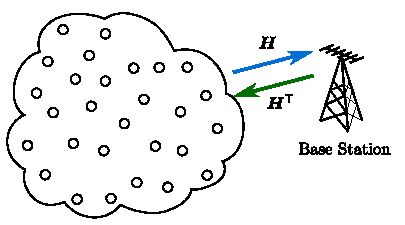
\includegraphics[width=0.5\textwidth]{./figs/system_figs/general_model.pdf}\\
	\caption{\textcolor{black}{Illustration of a large-scale network. Devices deliver (MAC, blue) or receive (BC, green) independent signals simultaneously on the same time-frequency resource.}}\label{system:fig:model}
\end{figure}

Note that due to the very nature of spatial diversity, up to $M$ users using the same resource can be independently served in downlink or uplink. Although methods such as successive interference cancellation (SIC) could help in servicing more users at a time, they are constrained by operation conditions (such as a significant power gap between signals), back-and-forth coordination and overhead (such as power control) and transceiver complexity (which is limited in IoT devices), and hence will not be considered in this dissertation.

In the following, we shall denote the uplink wireless MIMO channel as a complex matrix $\bm{H}$ of appropriate size, whose elements correspond to the transmitter-receiver antenna pairs formed by active devices and the BS. We assume a flat-fading channel that has no inter-symbol interference (ISI) during the link. 
As a single-carrier system, channel reciprocity ensures that the corresponding downlink MIMO channel matrix is $\bm{H}\T$.
The transmitted signal corresponding to user $u$ will be denoted by $s_u[k]$, where $k$ indicates the $k$-th symbol. $x_m[k]$ denotes the $k$-th symbol of the received signal (at the $m$-th BS antenna in the case of uplink), corresponding to the mixture of all transmitted signals through the MIMO channel. Finally, we use $y$ for the processed received signal, whose subindex will denote either the user (in downlink) or the recovered signal stream (in uplink).


\section{Blind Grant-Free Access}\label{system:sec:grant_free}
In uplink grant-free access, multiple signals could collide at the BS. In IoT applications, the energy and bandwidth consumption due to significant pilot overhead is undesirable, and we opt instead for blind signal recovery techniques.

Blind equalization has been a staple idea in terms of achieving this goal by diminishing the impact of pilots or preambles, aiming to reduce their impact in the overall bandwidth efficiency. 
Among blind equalization algorithms, the Constant Modulus Algorithm (CMA) presented by Godard \cite{Godard1980cma} in the 1980s is often considered the most widespread technique due to its computational simplicity and practical effectiveness \cite{Treichler1985,Ding2000}. We shall introduce the signal model for CMA-based signal recovery, and the current state of the art in solving the CMA formulation.

\subsection{CMA-based Blind Signal Recovery}\label{system:ssec:blind_recovery}
We consider the signal recovery of multiple users in one access group in a grant-free access system, as depicted in Figure~\ref{system:fig:general_model_access_control}. 
In particular, all potential uplink users in each access group have acquired network timing such that their uplink transmission bursts would span one given set of receiver time slots. 
Users in each designated access group may randomly transmit within their shared channel in terms of allocated resources. 
Appropriate coding and rate-matching is utilized by all source nodes to have equal number of data symbols $K$ within each access group and burst.
Furthermore, we design systems such that with very high probability or certainty the number of single-antenna active nodes $L$ shall fall below the number of diversity antennas $M$ at the receiver node. 
In particular, the receiver node does not necessarily know $L$.
Since the BS recovers multiple user signals during blind demixing without prior knowledge of their identities, the receiver can utilize user-ID scrambled CRC to check which recovered user signal belongs to which user, similar to the blind detection of PDCCH by users using RNTI-scrambled CRC in LTE or 5G \cite{ts36212,Jalali2020}. 

\begin{figure}[tbp]
	\centering
	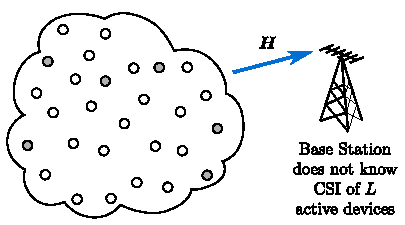
\includegraphics[width=0.5\linewidth]{./figs/system_figs/general_model_access_control.pdf}
	\caption{$L$ active sources (shaded gray) share a common resource block and transmit independent signals to the base station with $M$ antennas through an \emph{unknown} physical channel.}\label{system:fig:general_model_access_control}
\end{figure}

To summarize, we define the received signal vector $\xk$, the transmitted signal vector $\bm{s_k}$, and the flat fading channel $\bm{H}$, respectively, as 
\begin{align}
	\xk=\begin{bmatrix}
		x_1[k]\\\vdots\\x_M[k]
	\end{bmatrix},\, \bm{s}_k=\begin{bmatrix}
		s_1[k]\\\vdots\\s_L[k]
	\end{bmatrix},\,
	\bm{H}=\begin{bmatrix}
		h_{11}&\cdots&h_{1L}\\
		\vdots&\ddots&\vdots\\
		h_{M1}&\cdots&h_{ML}
	\end{bmatrix}.
	\label{system:eqn:signal_vectors}
\end{align}
Then the received signal vector at the BS can be written as
\begin{equation}
	\bm{x}_k=\bm{H}\bm{s}_k+\bm{n}_k, \label{system:eqn:rxsignal}
\end{equation}
where the (uplink) MIMO channel matrix $\bm{H}\in\mathbb{C}^{M\times L}$ is assumed to have full column rank $L$ (with $L\leq M$) and $\bm{n}_k\in\mathbb{C}^M$ is the vector of additive white Gaussian noises (AWGN) in that resource block, of the same size as $\xk$ in Eq.(\ref{system:eqn:signal_vectors}). Furthermore, and without loss of generality, we assume that all sources transmit equal average symbol energy $E_s=\mathbb{E}\big\{|s[k]|^2\big\}$. 
This assumption can be made as the different symbol energies of the sources $E_{s,\ell}$ can be included in the channel as $\bm{H}={\bm{H}'}\bm{D}^{1/2}$, with ${\bm{H}'}$ modeling only the channel fading across sources and receiver, and $\bm{D}=\diag(E_{s,1}/E_s,\ldots,E_{s,L}/E_s)$. Furthermore, note that although this signal model considers non-fading channels, the same formulation can be used for blind equalization by redefining the signal vectors and channel matrix \cite{Ding2000}.

Note that the receiver has explicit knowledge on neither the unknown channels $\bm{H}$ nor the number of active sources $L$, except for the statistical properties and the constellation of each source signal. 

\subsubsection{Recovering a Single Source}
When attempting to blindly recover one signal, the goal is to adaptively find a demixer such that its output corresponds to one of the transmitted signals with minimal interference, i.e.  
\begin{equation}
	{y}[k]=\w\herm \xk \approx \hat{s}_{\ell}[k],\quad	\ell\in\{1,\,\ldots,\, L\}. \label{system:eqn:ssr_demixer_output}
\end{equation}

The problem of blind signal recovery has been extensively studied before. In particular, Godard \cite{Godard1980cma} proposed what was later known \cite{Treichler1985} as the constant modulus algorithm (CMA) to find an optimum $\bm{{w}}\in\mathbb{C}^M$ by minimizing the mean CM cost for equalization:
\begin{equation}
	E\Big\{ \big(|y_k|^2 -R_2\big)^2\Big\}, \quad 
	R_2 = \frac{\mathbb{E}\{|s_\ell[k]|^4\}}{\mathbb{E}\{|s_\ell[k]|^2\}}, \label{system:eqn:cma_ssr_expectation}
\end{equation}
where the constant $R_2$ is computed from the high-order statistics of the source symbols $s[k]$ to match the input-output constellation scale \cite{Godard1980cma}.
It is known that CMA can be applied to i.i.d. signals using QAM constellations of arbitrary size and magnitude \cite{Ding2000}. 
Moreover, $R_2$ can be replaced by an arbitrary scalar, e.g. $1$, scaling $\bm{w}$ accordingly, and CMA will still converge such that its output recovers QAM source signals, without affecting signal integrity. 
In batch implementation, the single-source CM cost can be rewritten as 
\begin{equation}
	f(\w)=
	%\frac{1}{2K}\sum_{k=1}^K\Big(|y_k|^2-R_2\Big)^2 =
	\displaystyle{\frac{1}{2K}\sum_{k=1}^K\Big(|\xk\herm\w|^2-R_2\Big)^2},
	\label{system:eqn:cma_ssr}
\end{equation}
which is a smooth real-valued nonconvex function of $\w$. 
Note that $f$ presents phase invariance, i.e., if $\widehat{\w}$ is a solution that minimizes $f(\widehat{\w})$, then the entire set $\mathcal{W}({\widehat\w})=\{\e{j\theta}\widehat{\w}: \theta\in[0,2\pi]\}$ 
contains equivalent solutions that achieve the same minimum $f(\widehat{\w})$. 


\subsubsection{Simultaneous Multiple Signal Recovery}
In a more general setting, we are interested in deriving $J$ simultaneous demixers $\w_{\ell}\in\mathbb{C}^M$, $\ell\in\{1,\ldots,J\}$ that allow the recovery of $J$ sources with minimal interference, each tuned to a distinct signal. Without loss of generality, we consider $J\le L$.
We can also collect all demixers as columns of the receiver blind demixing matrix $\W=\big[\w_1\; \w_2\; \cdots \w_{\ell}\big]$, such that
\begin{equation}
	\bm{y}_{k}=\begin{bmatrix}
		\w_1\herm\\
		\vdots\\
		\w_{\ell}\herm\\
	\end{bmatrix}
	\xk= \W\herm \xk=
	\begin{bmatrix}
		\hat{s}_{\nu(1)}[k]\\
		\vdots\\
		\hat{s}_{\nu(\ell)}[k]\end{bmatrix},\quad
	\ell\in\{1,\,\ldots,\, J\},\;\nu(\ell)\in\{1,\ldots,L\}, \label{system:eqn:msr_demixer_output}
\end{equation}
where the permutation $\nu(\cdot)$ highlights that the BS has no prior knowledge of the identities of the transmitters.

CMA has been adapted in the past for simultaneous recovery of multiple independent source signals. 
In these applications, the first step is to define a cumulative demixing cost consisting of $J$ copies of CM costs, each one using a different demixer:
\begin{equation}
	f(\W)=
	%\frac{1}{2K}\sum_{\ell=1}^J\sum_{k=1}^K\Big(|y_{\ell}[k]|^2-R_2\Big)^2 =
	\displaystyle{\frac{1}{2K}\sum_{\ell=1}^J\sum_{k=1}^K\Big(|\xk\herm\w_{\ell}|^2-R_2\Big)^2}.
	\label{system:eqn:cma_msr_orig}
\end{equation}

The joint blind demixing problem is to optimize multiple solution vectors $\widehat\W=\big[\widehat{\w}_1\;\cdots\;\widehat{\w}_{\ell}\big]$ that jointly minimize the cumulative CM cost of (\ref{system:eqn:cma_msr_orig}). 
Note that this cumulative CM cost by itself cannot guarantee that the recovered signals are indeed from different sources. 
In fact, even if every one column vector of $\widehat \W$ captures the same signal source, the cumulative CM cost of (\ref{system:eqn:cma_msr_orig}) is still minimized and cannot prevent such solutions. 
For this reason, it is clear that the cumulative CM cost of (\ref{system:eqn:cma_msr_orig}) is non-convex and is in fact multi-modal. 
%Hence, the challenge lies in the practical need that distinct source signals be recovered by the $J$ solution vectors of $\widehat \W$. 
%Additionally, we need to ensure that the demixers do not merely restore the same source signal for only a small subset of sources, possibly with different phases or delays \cite{Ding2000}. 
Therefore, when considering simultaneous multiple signal recovery, additional constraints must be enforced for demixers $\w_{\ell},\,\ell\in\{1,\ldots,J\}$ to recover different source signals. 






\subsection{Constant Modulus Algorithm}\label{system:ssec:cma}

%presentation

Among blind equalization algorithms, CMA \cite{Godard1980cma} is often considered the most widespread blind technique due to its computational simplicity and practical effectiveness, as its independence of carrier recovery \cite{Ding2000}. It is also well-known that it enjoys global convergence properties in noiseless scenarios under full rank channel conditions \cite{LiDing1994cmaglobalconvergencefse}. 

% classical CMA and drawbacks
Traditionally, CMA is implemented using stochastic gradient descent and variations. 
However, one of its major issues in its practical applications is the presence of local minima in the constant modulus (CM) cost function as a result of additive channel noise \cite{Fijalkow1998,Chung1998}. 
The convergence properties of such stochastic gradient descent algorithms have not been fully understood under limited samples and additive channel noise \cite{Ding2000,Zeng1999analysiscma,Dabeer2003convergencecma}.  
Moreover, the stochastic gradient descent approach has fundamental tradeoffs and requires finely tuning of e.g., initialization, normalization and stepsize, for satisfactory convergence and decent speed. 

%
% semidefinite relaxation CMA
Several works have proposed different approaches that try to overcome these inherent shortcomings.
%
One interesting approach is the transformation of CMA-based equalization to a convex problem, via Semidefinite relaxation \cite{Mariere2003BlindCM,Luo2004sdrquadratic,Wang2018sdrbe}, which provides  global convergent solutions in a lifted higher dimensional parameter space that are further projected to the original solution space. 
As with any relaxation approach, CMA based on convex relaxation relies on the expectation that the convex problem yields solutions that can be projected to near optimum CMA solutions. However, projecting back to the original parameter space via rank 1 decomposition remains difficult and elusive \cite{Adler2019nuclearnorm}.
Additionally, the problem size grows polynomially with increasing parameter size of the linear system and multiple users, and poses severe practical challenges in many scenarios. 
%

% analytical CMA
Other line of works tries to solve CMA problems analytically \cite{Hassibi1994closedformcma,vanderVeen1996acma}. These solutions and its variants \cite{vanderVeen2005adaptiveacma,Zarzoso2008optimalstepsizecma}, have no convergence issues as the solutions are found algebraically.
However, they are more complex in general, and usually require stricter assumptions, such as constant modulus constellations, and cannot work with general QAM source signals such as 16-QAM. 
There are also multistage schemes \cite{Shynk1994performancemultistagecma}, that depend heavily on the estimation error being close to the MMSE estimate in earlier stages, or the error accumulates through different stages \cite{Liu1999cmaarray}. 
%Now, considering blind recovery of multiple sources, one could try to minimize the CM cost in hope of recovering one individual output each time. One could use successive interference cancellation (SIC) to remove the recovered signal contribution from the received signal $\bm{x}_k$ before minimizing the CM cost again to recover another signal. However, SIC has a well-known shortcoming of error propagation. 
%

% MSR
Moreover, several CMA-based approaches have been proposed to enforce the recovery of multiple signals at a time. 
One family of solutions is to consider regularization terms in the cost function \cite{Bessios1992mimocrimno,Li1998adaptivemimocma,Ikhlef2007simplifiedmimocma}, which enforce the recovered signals to be uncorrelated. 
Other schemes propose to modify the iterate after the gradient descent update, such as performing an iterative orthogonality enforcement on the combiners \cite{Nguyen1997}. 
In general, these approaches are slow, as they require a rather large amount of samples and/or iterations to attain sufficient interference rejection of all recovered sources.


% nonconvex
A new line of research is delivering algorithms to directly solve nonconvex optimization problems, and have been successfully applied in different domains, such as phase retrieval \cite{Candes2015a_phaseretrievalWF,Candes2013}, matrix completion \cite{Keshavan2010matrixcompletion,Yang2016lowrankfogran}, blind deconvolution \cite{Dong2018blinddemixingwf}, among others.
These are attractive solutions, as they do not require a prohibitive problem size or approximate relaxations, and provide good results with reasonable complexity and sample efficiency.
Thus, these techniques can be better suited for grant-free access in resource limited networks.
In Chapter~\ref{wfcma:chap}, we adapt these results to the CMA-based signal recovery problem. By applying the Wirtinger Flow \cite{Candes2015a_phaseretrievalWF}, we provide theoretical convergence guarantees in the finite-sample regime for both single and multiple source recovery, and demonstrate the efficiency of this methods via numerical simulations. 


% Riemann
In a separate line of work, Riemannian manifold optimization \cite{Absil2008book} has rapidly attracted interest due to its ability to tackle non-convex problems with reasonable computational cost, and has been successfully applied to several domains, such as low-rank matrix decomposition \cite{Yang2016lowrankfogran}, singular value decomposition \cite{Sato2014complexstiefel}, phase retrieval \cite{Huang2016phaseliftriemann}, blind signal demixing \cite{Dong2019blinddemixingrtr}, dictionary learning \cite{Cherian2015riemanniandictionary,Sun2017riemanniandictionary}, among many others.
In this framework, a constrained optimization problem in Euclidean space is transformed into an unconstrained problem over a Riemannian manifold, a subset of Euclidean space with nice properties. 
As the manifold contains only the interesting search directions for the problem, this approach potentially reduces computation. Moreover, it can avoid directions of invariance of the cost function, significantly facilitating theoretical analysis and direct application of optimization techniques. 
%More importantly, manifold optimization can help providing certain guarantees of convergence of first and second order optimization methods, as directions of invariance of the cost function can also be discarded altogether. 
We show in Chapter~\ref{wfcma:chap} our application of the Riemannian manifold optimization framework to CMA-based signal recovery. By defining an adequate Riemannian manifold, we provide a non-regularized approach for multiple signal recovery that enjoys convergence guarantees with second order methods. Our experiments show excellent signal recovery capabilities with low sample complexity and computational complexity, and presents the Riemannian framework as a promising direction to the improvement of grant-free communications. 





\section{User Scheduling} \label{system:sec:usch}

We now consider a user scheduling scenario as depicted in Figure~\ref{system:fig:general_model_user_sch}. We assume that the BS knows the CSI of all $N$ active devices (also denoted users), and therefore the BS shall manage user scheduling, in both uplink (MAC) and downlink (BC). We further assume that the users only know their own CSI.
\begin{figure}[tbp]
	\centering
	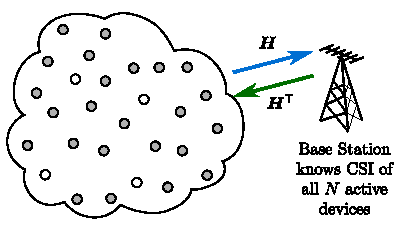
\includegraphics[width=0.5\linewidth]{./figs/system_figs/general_model_user_sch.pdf}
	\caption{$N$ active users (shaded gray) share a common resource block and transmit (MAC, blue) or receive (BC, green) independent signals simultaneously through a \emph{known} physical channel.}\label{system:fig:general_model_user_sch}
\end{figure}

Without loss of generality, we consider MIMO systems that leverage spatial diversity to accommodate spectrum-sharing user groups allocated into distinct resources in multiple access strategies such as OFDMA and TDMA, among others. As stated before, we impose that resource-sharing groups (RSGs) shall have at most $M$ users, to ensure linear independence of user CSIs within each group.

In agreement with the general model of Section~\ref{system:sec:model}, $\bm{h}_{u}\in \mathbb{C}^{M}$ and $\bm{h}_u\T$ denote the uplink and downlink CSI vector of the $u$-th user, respectively, with $u\in\{1,\ldots,N\}$. We assume the CSIs are random and independent from each other. We let $s_{u}$ denote the $u-$th user data symbol of zero mean and unit average power, i.e. $\mathbb{E}\left[ {|{s_{u}}|^2} \right] = 1$. 
Let $G$ the total number of groups to be assigned, and let $\pi_{g,u}\in\{0,1\}$ indicate whether the $u$-th user is scheduled in group $g\in\{1,\ldots,G\}$ exclusively, i.e.
\begin{equation}
	{\pi _{g,u}} = \left\{ \begin{array}{ll}
		1&\text{the $u$-th user belongs to group $g$ only,}\\
		0&\text{otherwise,}
	\end{array} \right.
\end{equation}
% and  $\bm{\Pi}_g=\diag(\pi_{g,1},\ldots,\pi_{g,N})\in\{0,1\}^{N\times N}$ the matrix that collects all indicators of group $g$ in its diagonal.
and the set $\mathcal{S}_g=\{u|\pi_{g,u}=1, u\in\{1,\ldots,N\}\}$ denotes the scheduled user set of the $g$-th group with cardinality $|\mathcal{S}_g|$.
% Finally, we define $\bm{\Pi}=\{\bm{\Pi}_g\}_{g=1}^G$ as the set of indicator matrices.
As the BS manages user scheduling, it also manages the transmit power allocated to each user, denoted $p_u$.

\subsection{Uplink (MAC) Model} \label{system:ssec:usch_mac}

At the BS, the $|\mathcal{S}_g|$ user signals from the scheduled MAC user group $g$ arrive at the BS receiver through their respective channel responses $\{\bm{h}_u\}_{u\in\mathcal{S}_g}$, which are then decoded using a linear receiver $\bm{W}_g$ such as the MRC, ZF and MMSE receivers \cite{Tse05}, to generate the decoded signal vector
\begin{align}\label{system:eqn:usch_sig_mac}
	\bm{y}_g^{\MAC}&= \bm{W}_g\herm\bigg(\sum\nolimits_{u \in \mathcal{S}_g} \bm{h}_u\sqrt {p_{u}}s_{u}  + \bm{n}_g\bigg)
	% 	\nonumber\\&
	=\bm{W}_g\herm\bigg(\sum\nolimits_{n=1}^N \bm{h}_u\sqrt {p_{u}}s_{u}\pi_{g,u}  + \bm{n}_g\bigg)
	% 	\nonumber\\
	% 	&=\bm{Q}_g\herm\bm{H}\bm{\Pi}_g\bm{P}^{1/2}\bm{x} + \bm{Q}_g\herm\bm{w}_g,
	% 	&= \bm{H}\bm{P}^{1/2}\bm{\Pi}_{g}\bm{x}  + \bm{w}_g
\end{align}
where 
% $\bm{x}=\begin{bmatrix} x_1&\cdots &s_n \end{bmatrix}\T$ is the vector containing the symbols transmitted by all users, and 
$\bm{n}_g\sim \mathcal{CN}(\bm{0}_M,\sigma^2 \bm{I}_{M})$ represents the AWGN vector corresponding to the resource block assigned to group $g$.
%\textcolor{magenta}{Here we can see that the dimension of $\bm{y}_g$, $N_0=\text{rank}(\bm{H}_g)\leq \min(M,N)$ is the number of parallel streams of data that is to be transmitted \cite{Sampath01}.}
%\cjferes{This is not true. The size of $\bm{y}$ will be dictated by the number of BS antennas, and it does not say a thing about the rank of the channel matrix. We can say $N_0=\mathrm{rank}$ if we want, but it does not relate necessarily to the received vector size.}
%  with zero mean and covariance matrix of $\sigma^2 {\bm{I}}_{N}$.\
% this commented part is redundant.
% \begin{subequations}
	% \begin{align}
		% \bm{H}_g&=\left[ {{{\bm{h}}_{m}}|\pi_{g,m}=1,\forall m} \right]_{{N {\times } {|\mathcal{S}_g|}}},\\
		% \bm{P}_g &=\text{diag}\left(\sqrt{p_m}|\pi_{g,m}=1,\forall m\right),\\
		% \bm{x}_g&=\left[{x_m|\pi_{g,m}=1,\forall m}\right]_{{|\mathcal{S}_g|}\times 1},
		% \end{align}
	% \end{subequations}
% and we can rewrite the MAC signal model (\ref{usch:eqn:sig_mac}) as
% \begin{align}
	% 	\bm{y}_g^{\MAC} = \bm{H}_g\bm{P}^{1/2}\bm{x} + \bm{w}_g.
	% 	\label{usch:eqn:sig_mac_2}
	% \end{align}
% \textcolor{blue}{Note that the model in (\ref{usch:sig}) is indeed very general and widely used in MIMO systems.}

\subsection{Downlink (BC) Model} \label{system:ssec:usch_bc}

In the case of BC, we operate under equal assumptions. However, the signal model changes as the single-antenna receivers will experience CCI but will not be aware of the CSI of other users in the RSG. Furthermore, the received signal and noise are scalars, and the BS uses a linear, unitary beamforming precoder $\bm{z}_u$ for each user $u$, which can be selected as the weighted MMSE \cite{Bjornson2013wmmsebc}, MRT \cite{Lo1999mrt} or ZF precoder \cite{Jindal206zfbc} among others. For notational simplicity, we abuse notation and we use $g$ to also denote the group index of the group that contains user $u$.
% whenever the user $n\in\mathcal{S}_g$, $g$ let $g(n)$ denote the group index for the group that contains user $n$, that is, $n\in\mathcal{S}_{g(n)}$.
Therefore, the signal model for the signal that user $u$ receives in BC mode with AWGN $n_u\sim\mathcal{CN}(0,\sigma^2)$ corresponds to:
\begin{align}\label{system:eqn:usch_sig_bc}
	{y}_n^{\BC}
	% 	&= \bm{h}_n\herm\bm{z}_n\sqrt{p_n} x_{n}+\sum\nolimits_{i \in \mathcal{S}_g,i\neq n} \bm{h}_i\herm\bm{z}_{i}\sqrt {p_{i}}x_i  + {w}_n.
	&= \bm{h}_u\T\sum\nolimits_{i \in \mathcal{S}_{g}}\bm{z}_i\sqrt{p_i} s_{i}  + {n}_u
	% 	\nonumber\\&
	= \bm{h}_u\T\sum\nolimits_{i=1}^N\bm{z}_i\sqrt{p_i} s_{i}\pi_{g,i}  + {n}_u.
	% 	&= \bm{H}\bm{P}^{1/2}\bm{\Pi}_{g}\bm{x}  + \bm{w}_g
\end{align}



\subsection{State of the Art}\label{system:ssec:usch_stateart}

Given a large number of serviced devices $N$ and increasing large number of base-station antennas $M$, the number of user scheduling options is of order $\mathcal{O}(N^M)$. 
Thus, to optimally schedule users in resource-sharing groups, one needs to examine the CSIs of each possible user grouping among potentially very large number of users in e.g., the thousands. However, since MIMO user scheduling is a combinatorial, NP-hard problem, even for a moderate number of users (e.g. hundreds), it is difficult to exhaustively evaluate all possible user combinations as MIMO user groups against one or more objectives.

Therefore, algorithms typically rely on heuristics when the user number becomes very large as in the case of IoT. 
For example, some recent methods take advantage of proportional fairness (PF) and the determinant pairing algorithm (DPS) \cite{Chen08, Chang16, wang11}. 
However, these schemes rely on exhaustive computation of spatial cross-correlations for various possible user groups, and as such still require heavy computational workload.

Other approaches exploit localized characteristics shared among small subsets of users. One proposal examines $N(N-1)/2$ pairwise CSI correlations among all $N$ users and proposes to form user groups by setting a maximum correlation threshold \cite{Zhang05, Kim15}. 
Other schemes such as \cite{Dhanushka19, Sharath19} directly group users of similar CSI covariance matrices.  
Nevertheless, information on pairwise or small user subsets fail to capture broad comprehensive characteristics on the entire user set. 
In the case of pairwise correlation, e.g., multiple users with low pairwise correlation in an MIMO user group may still suffer from significant interference accumulation. 
Localized approaches are also very sensitive to choices of manual parameter tuning and are harder to scale, as different choices might lead to drastically different performance as the user number changes or as the CSI models vary. 

Recently, (machine) learning based approaches have been applied to a diverse array of difficult networking problems, including MAC user scheduling \cite{Jiang17, Morocho19, Xu14, Cui18}. 
In fact, both supervised and unsupervised learning algorithms have found applications in wireless CSI characterization \cite{Jiang17} that could be utilized in MIMO user scheduling.
Machine learning is particularly attractive for large, NP-hard problems such as user scheduling that would require very high complexity to solve directly.
In the context of wireless networking, supervised learning requires a rich labeled training set of diverse CSIs and correspondingly optimized scheduled user groups that attain strong performance. 
Such labeled training set must account for different system conditions such as number of antennas, number of users, wireless channel characteristics, noise levels, different power constraints, among others.
However, it is not practically feasible to build such a huge set of optimum solutions. 
Ironically, supervised learning itself cannot be trained to find such optimum solutions for training.

In contrast, unsupervised learning explores underlying data features and characteristics without relying on labeled training set.
Importantly in the context of large-scale user scheduling, unsupervised learning can effectively identify users with highly similar CSIs, as proposed for direct user grouping in downlink multi-cast \cite{Xu14, Cui18}. 
However, for the more general multi-user MIMO systems operating in either uplink MAC or downlink BC (also known as MU-MIMO), scheduling users with similar CSI leads to poor joint spatial diversity.
Such outcome deviates from the original goal of diversity-based user scheduling, aimed at scheduling users with highly dissimilar CSIs into MIMO co-channel groups to promote spatial diversity and to mitigate mutual interference. 
Clearly, a direct application of traditional learning algorithms over CSI vectors is incompatible with the MIMO user scheduling task. 
Additionally, unsupervised learning is often based in Euclidean space, but Euclidean distance of CSI does not correspond to spatial diversity as the latter is related to subspace span. 

In the second part of this dissertation (Chapter~\ref{usch:chap}), we propose a novel approach that leverages unsupervised learning to indirectly allocate users into RSGs. We will show that this strategy provides significant performance gains with modest computational cost, and can be generalized to consider a variety of performance metrics and different algorithms to further improve its results. 


